\documentclass[11pt]{article}
\usepackage{geometry}
\usepackage[spanish]{babel}
\usepackage[utf8]{inputenc}
\usepackage{tocloft}
\usepackage{graphicx}
\usepackage{ragged2e}
\usepackage{natbib}
\usepackage{amsmath}
\usepackage{amsfonts}
\renewcommand{\thesection}{\arabic{section}}
\geometry{
    left=3cm,
    right=3cm,
    top=2.5cm,
    bottom=2.5cm
}
\linespread{1.2}

\usepackage[colorlinks=true, allcolors=blue]{hyperref}
\hypersetup{
    colorlinks=true,% make the links colored
}
\usepackage{appendix}
\usepackage{adjustbox}
\usepackage{float}
\usepackage{booktabs}
\usepackage{multirow}
\usepackage{color}
\usepackage{rotating}
\usepackage{fancybox}
\usepackage{lscape}
\usepackage{makecell}
\usepackage{graphicx}
\usepackage{ltablex}



\begin{document}   


\begin{titlepage}
    \centering
    \vspace*{2cm}
    
\includegraphics[width=1\textwidth]{logo.png} 
    
    \vspace{2cm}
    {\scshape\LARGE Maestría en Economía} \\
    
    \vspace{0.5cm}
    {\huge\bfseries
    Trabajo Práctico\par}
    \vspace{2cm}
    {\Large\itshape Coloma Conte-Grand, Carolina} \\
    
    {\Large\itshape Condori, Brayan Alexis} \\
    
    {\Large\itshape Deniard, Agustín}
    \vfill
    {\Large Profesor: Javier Alejo} \\
    \vspace{0.5cm}
    {\Large Materia: Regresiones por Cuantiles}

    \vfill

    {\large \today\par}
\end{titlepage}

\justify 

\section*{Ejercicio 1}


El cuadro \ref{tab:sum_stats} muestra las estadísticas descriptivas de las variables explicativas de la ecuación de Mincer. La muestra total incluye a 7,903 individuos entre 18 y 65 años que residen en Gran Buenos Aires. Para los ingresos horarios de la ocupación principal, observamos una tendencia creciente en la mediana a medida que aumenta la edad. En todos los grupos de edad, existe una brecha entre los individuos del primer y el último decil, siendo más pronunciado en el grupo de 65 años, aunque este grupo tiene una muestra pequeña (80 obs.). Excluyendo este grupo, el rango de personas entre 41 y 64 años muestra la mayor disparidad, con el último decil (91.0) casi seis veces superior al primero (15.5). Respecto a los años de educación recibidos, se observa un patrón similar entre el primer y último decil, con la mayor brecha en los grupos etarios de 25-40 y 41-64 años, excluyendo a los de 65 años. Sin embargo, los años de educación recibidos por individuo mediano en cada grupo etario es de 12 años, excepto para el grupo de 65 años, donde es 11 años. Finalmente, la muestra incluye un 42.2\% de mujeres y un 26.6\% de residentes en CABA


\begin{table}[H]
    \centering
    \caption[Estadísticas descriptivas]{Estadísticas descriptivas}
    \label{tab:sum_stats}
    \begin{adjustbox}{max width=\textwidth}
        \begin{tabular}{l*{2}{c}}
            
\begin{tabular}{l*{15}{c}}
\hline\hline
 & \multicolumn{6}{c}{} & \multicolumn{7}{c}{\centering Deciles} \\ \cmidrule(lr){7-15}
 & N & Media & SD & Min & Max & 10 & 20 & 30 & 40 & 50 & 60 & 70 & 80 & 90  \\
\hline
\textit{Ingreso horario en la ocupaci�n principal} \\
\hspace{0.25cm} Grupo de edad: [15,24] & 998 &  34.5 &  28.8 &   0.6 & 515.5 &  13.5 &  18.2 &  21.9 &  25.8 &  30.2 &  33.4 &  37.6 &  43.3 &  60.1 \\
\hspace{0.25cm}  Grupo de edad: [25,40] & 3339 &  47.6 &  46.5 &   0.6 & 1804.1 &  17.2 &  24.3 &  29.1 &  34.4 &  39.4 &  45.1 &  52.0 &  64.4 &  85.0 \\
\hspace{0.25cm}  Grupo de edad: [41,64] & 3486 &  49.3 &  44.5 &   0.2 & 827.4 &  15.5 &  22.1 &  27.8 &  33.1 &  39.4 &  45.5 &  53.5 &  64.7 &  91.0 \\
\hspace{0.25cm}  Grupo de edad: [65+] & 80 &  58.5 &  89.0 &   4.6 & 618.6 &  11.4 &  15.4 &  24.2 &  28.8 &  36.2 &  42.2 &  48.5 &  68.7 & 113.5 \\
\textit{Años de educación} \\
\hspace{0.25cm} Grupo de edad: [15,24] & 998 &  11.2 &   2.6 &   2.0 &  17.0 &   7.0 &   9.0 &  10.0 &  12.0 &  12.0 &  12.0 &  12.0 &  13.0 &  14.0 \\
\hspace{0.25cm}  Grupo de edad: [25,40] & 3339 &  12.2 &   3.4 &   0.0 &  20.0 &   7.0 &   9.0 &  11.0 &  12.0 &  12.0 &  12.0 &  15.0 &  15.0 &  17.0 \\
\hspace{0.25cm}  Grupo de edad: [41,64] & 3486 &  11.2 &   4.0 &   0.0 &  20.0 &   7.0 &   7.0 &   7.0 &  10.0 &  12.0 &  12.0 &  14.0 &  15.0 &  17.0 \\
\hspace{0.25cm}  Grupo de edad: [65+] & 80 &  10.7 &   4.8 &   0.0 &  19.0 &   4.5 &   7.0 &   7.0 &   7.0 &  11.0 &  12.0 &  15.0 &  16.5 &  17.0 \\
\textit{Edad} \\
\hspace{0.25cm} Grupo de edad: [15,24] & 998 &  21.6 &   1.8 &  18.0 &  24.0 &  19.0 &  20.0 &  21.0 &  21.0 &  22.0 &  22.0 &  23.0 &  23.0 &  24.0 \\
\hspace{0.25cm}  Grupo de edad: [25,40] & 3339 &  32.6 &   4.6 &  25.0 &  40.0 &  26.0 &  28.0 &  30.0 &  31.0 &  33.0 &  34.0 &  36.0 &  37.0 &  39.0 \\
\hspace{0.25cm}  Grupo de edad: [41,64] & 3486 &  51.1 &   6.8 &  41.0 &  64.0 &  42.0 &  44.0 &  46.0 &  48.0 &  51.0 &  53.0 &  55.0 &  58.0 &  61.0 \\
\hspace{0.25cm}  Grupo de edad: [65+] & 80 &  65.0 &   0.0 &  65.0 &  65.0 &  65.0 &  65.0 &  65.0 &  65.0 &  65.0 &  65.0 &  65.0 &  65.0 &  65.0 \\
Mujer (=1) & 7903 & 0.422 & 0.494 & - & - & - & - & - & - & - & - & - & - & - \\
Reside en CABA (=1) & 7903 & 0.266 & 0.442 & - & - & - & - & - & - & - & - & - & - & - \\
\hline\hline \multicolumn{15}{p{20cm}}{}\\ 
\end{tabular}
        \end{tabular}
    \end{adjustbox}
\end{table}

El cuadro \ref{tab:OLS_mincer} muestra los resultados de la estimación de la ecuación de Mincer mediante OLS. Dado que el efecto marginal no es constante para las variables de edad y educación, tomamos como referencia a un individuo de 30 años de edad y 12 años de educación formal. Un incremento de un año en la edad se asocia con un aumento promedio del 1.36\% en el ingreso laboral horario, mientras que un incremento de un año de educación se asocia con un aumento promedio del 8.50\%. Por otro lado, ser mujer se asocia con una reducción promedio del 13.27\% en el ingreso laboral horario en comparación con ser hombre. Por último, residir en CABA se asocia con un aumento promedio del 14.53\% en el ingreso laboral horario, respecto a quienes viven en el Conurbano Bonaerense. Todos los resultados descritos son significativos al 1\%.
\begin{table}[H]
    \centering
    \caption[Estimación de la ecuación de Mincer por MCO]{Estimación de la ecuación de Mincer por MCO}
    \label{tab:OLS_mincer}
    \begin{adjustbox}{max width=0.8\textwidth}
        \begin{tabular}{l*{2}{c}}
            {
\def\sym#1{\ifmmode^{#1}\else\(^{#1}\)\fi}
\begin{tabular}{l*{1}{D{.}{.}{-1}}}
\toprule
                &Salario horario (log)         \\
                &\multicolumn{1}{c}{(1)}         \\
\midrule
Años de educación&   -0.039\sym{***}\\
                &  (0.010)         \\
\addlinespace
Años de educación $\times$ Años de educación&    0.005\sym{***}\\
                &  (0.000)         \\
\addlinespace
Edad            &    0.035\sym{***}\\
                &  (0.004)         \\
\addlinespace
Edad $\times$ Edad&   -0.000\sym{***}\\
                &  (0.000)         \\
\addlinespace
Mujer (=1)      &   -0.142\sym{***}\\
                &  (0.015)         \\
\addlinespace
Reside en CABA (=1)&    0.136\sym{***}\\
                &  (0.017)         \\
\addlinespace
Constant        &    2.534\sym{***}\\
                &  (0.097)         \\
\bottomrule
\multicolumn{2}{l}{\footnotesize Standard errors in parentheses}\\
\multicolumn{2}{l}{\footnotesize \sym{*} \(p<0.10\), \sym{**} \(p<0.05\), \sym{***} \(p<0.01\)}\\
\end{tabular}
}

        \end{tabular}
    \end{adjustbox}
\end{table}


\section*{Ejercicio 2}

El cuadro \ref{tab:QR_Mincer} presenta las estimaciones de los coeficientes del modelo para el $\tau$-ésimo cuantil condicional de la ecuación de Mincer:
\[
Q_{\tau}(y|x)\;=\;x_{i}^{T}\beta(\tau)
\]
en donde $\tau\in\{0.05,0.25,0.50,0.75,0.95\}$, $y$ es el logaritmo natural del ingreso laboral por hora y $x$ es el vector de variables explicativas para esta especificación de la ecuación de Mincer, conformada por los años de educación (y su cuadrado), la edad (y su cuadrado), el sexo y la ubicación geográfica. Dado que el efecto marginal no es constante para las variables de edad y educación, tomamos como referencia a un individuo de 30 años de edad y 12 años de educación formal.
\begin{itemize}
    \item Con $\tau=0,05$:
    \begin{itemize}
        \item Un año adicional de educación para una persona con 12 año de educación formal se traduce, \emph{ceteris paribus}, en un aumento del 9,76\% en el ingreso laboral horario del cuantil 0,05.
        \item Un año adicional de edad para una persona de 30 años se traduce, \emph{ceteris paribus}, en un aumento del 0,82\% en el ingreso laboral horario del cuantil 0,05.
        \item El ingreso laboral horario del cuantil 0,05 es un 27,6\% menor para las mujeres en comparación con los hombres.
        El ingreso laboral horario del cuantil 0,05 es un 36,48\% mayor para quienes residen en Capital Federal en comparación con aquellos que viven en el conurbano bonaerense.
    \end{itemize}
    Los coeficientes que acompañan a las variables \emph{caba} y \emph{female} son significativos al 1\%, mientras que los que acompañan a la variable \emph{edad} (tanto para el término lineal como para el cuadrático) son significativos al 5\%.
    \item Con $\tau=0,25$:
    \begin{itemize}
        \item Un año adicional de educación para una persona con 12 año de educación formal se traduce, \emph{ceteris paribus}, en un aumento del 8,69\% en el ingreso laboral horario del cuantil 0,25.
        \item Un año adicional de edad para una persona de 30 años se traduce, \emph{ceteris paribus}, en un aumento del 1,41\% en el ingreso laboral horario del cuantil 0,25.
        \item El ingreso laboral horario del cuantil 0,25 es un 10,95\% menor para las mujeres en comparación con los hombres.
        El ingreso laboral horario del cuantil 0,25 es un 12,41\% mayor para quienes residen en Capital Federal en comparación con aquellos que viven en el conurbano bonaerense.
    \end{itemize}
    \item Con $\tau=0,5$:
    \begin{itemize}
        \item Un año adicional de educación para una persona con 12 año de educación formal se traduce, \emph{ceteris paribus}, en un aumento del 8,04\% en el ingreso laboral horario del cuantil 0,5.
        \item Un año adicional de edad para una persona de 30 años se traduce, \emph{ceteris paribus}, en un aumento del 1,5\% en el ingreso laboral horario del cuantil 0,5.
        \item El ingreso laboral horario del cuantil 0,5 es un 11,75\% menor para las mujeres en comparación con los hombres.
        El ingreso laboral horario del cuantil 0,5 es un 13,09\% mayor para quienes residen en Capital Federal en comparación con aquellos que viven en el conurbano bonaerense.
    \end{itemize}
    \item Con $\tau=0,75$:
    \begin{itemize}
        \item Un año adicional de educación para una persona con 12 año de educación formal se traduce, \emph{ceteris paribus}, en un aumento del 8,51\% en el ingreso laboral horario del cuantil 0,75.
        \item Un año adicional de edad para una persona de 30 años se traduce, \emph{ceteris paribus}, en un aumento del 1,48\% en el ingreso laboral horario del cuantil 0,75.
        \item El ingreso laboral horario del cuantil 0,75 es un 12,1\% menor para las mujeres en comparación con los hombres.
        El ingreso laboral horario del cuantil 0,75 es un 10\% mayor para quienes residen en Capital Federal en comparación con aquellos que viven en el conurbano bonaerense.
    \end{itemize}
    \item Con $\tau=0,95$:
    \begin{itemize}
        \item Un año adicional de educación para una persona con 12 año de educación formal se traduce, \emph{ceteris paribus}, en un aumento del 8,31\% en el ingreso laboral horario del cuantil 0,95.
        \item Un año adicional de edad para una persona de 30 años se traduce, \emph{ceteris paribus}, en un aumento del 1,19\% en el ingreso laboral horario del cuantil 0,95.
        \item El ingreso laboral horario del cuantil 0,95 es un 10,15\% menor para las mujeres en comparación con los hombres.
        El ingreso laboral horario del cuantil 0,95 es un 14,91\% mayor para quienes residen en Capital Federal en comparación con aquellos que viven en el conurbano bonaerense.
    \end{itemize}
\end{itemize}
En todos los casos, los coeficientes que acompañan a las variables \emph{caba}, \emph{female} y son significativos al 1\%. Por su parte, los coeficientesque acompañan a la variable \emph{edad} (tanto para el término lineal como para el cuadrático) son simpre significativos pero a distintos niveles de significatividad. Finalmente, los coeficientes que acompañan a la variable \emph{edad} son siempre significativos para el término cuadrático (aunque a distintos niveles de significatividad), pero no para el término lineal (que es no significativo para los cuantilies 0,05 y 0,25). 

\section*{Ejercicio 3}

Realizamos un test para estudiar si el efecto parcial de los años de educación sobre el salario es el mismo para los cuantiles condicionales 0.05 y 0.95. Encontramos que el p-valor asociado es de 0,0452, lo cual resulta significativo a 0,05 y nos permite rechazar para este nivel la hipótesis nula de que el efecto parcial de la educación sobre el salario es el mismo en ambos cuantiles.

A su vez, realizamos un test bajo la hipótesis nula de que los coeficientes del modelo (a excepción de la ordenada al origen) no difieren entre cuantiles condicionales. Encontramos que el p-valor asociado es casi nulo, por lo que podemos rechazar la hipótesis nula para un nivel de 0,0001. 

Este test es útil para estudiar la relevancia del modelo ya que muestra si existe o no información adicional proveniente de las regresiones por cuantiles. Si la hipótesis nula no fuera rechazada, esto implicaría que los efectos parciales son iguales sin importar el cuantil, por lo que no habría diferencia entre la información proporcionada por una estimación cuantílica y la obtenida en una regresión por MCO.

\section*{Ejercicio 4}

Graficamos los coeficientes de la regresión en función a los cuantiles $\tau$ estimados. Encontramos que en general todos difieren respecto de la estimación de OLS, aunque esta recta suele encontrarse contenida en la mayoría de los intervalos de confianza estimados por bootstrap. 

\begin{figure}[H]
	\caption{Coeficientes de la regresión respecto al cuantil $\tau$}
	\centering
	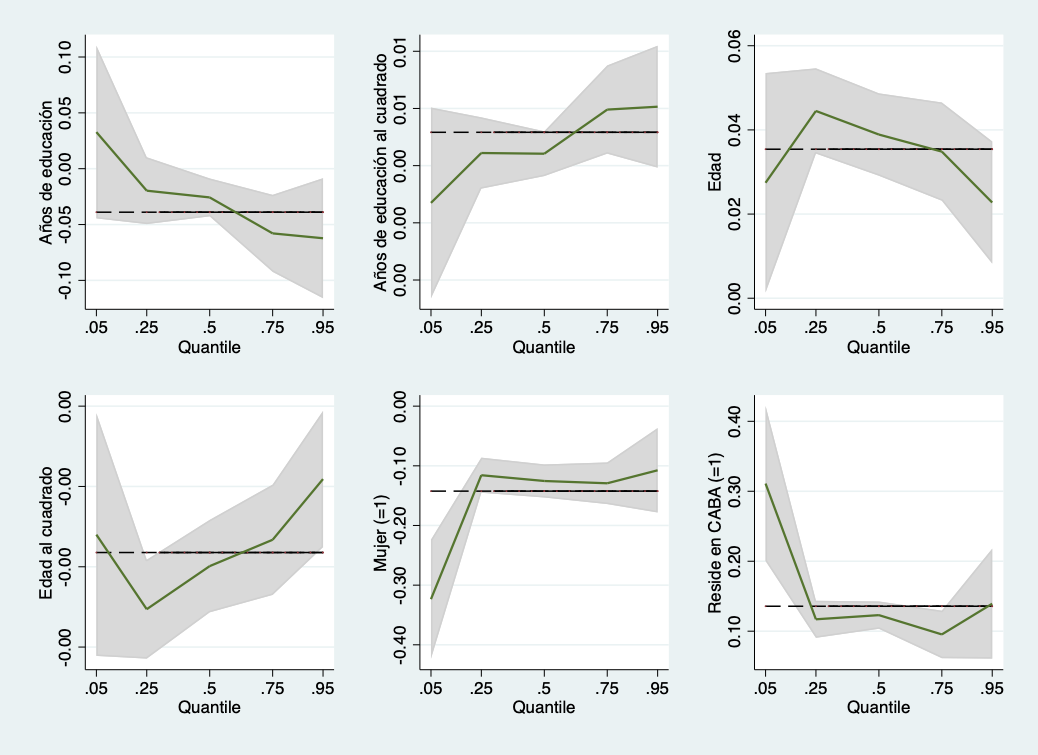
\includegraphics[width=0.8\linewidth]{4.png}
\end{figure}

El método de regresiones por cuantiles es considera uno semiparamétrico. Tiene un componente paramétrico ya que modela a los cuantiles condicionales de la variable dependiente suponiendo una estructura lineal $Q_y(\tau | X ) = X \beta(\tau)$. A su vez, tiene un componente no paramétrico en que no asume una distribución específica para los errores estándares y estima los cuantiles condicionales a partir de la forma de los datos. Por esto se dice que es un método \textit{distribution free}.

\section*{Ejercicio 5}

\begin{table}
    \centering
    \begin{tabular}{|c|c|c|c|}
    \hline
         & \textbf{Q25} & \textbf{Q50} & \textbf{Q75}\\ \hline
    Negativo & 1.972 (24,95\%) & 3.946 (49,93\%) & 5.924 (74,96\%) \\
    Nulo     & 8 (0,10\%) & 8 (0,10\%) & 7 (0,09\%) \\
    Positivo & 5.923 (74,95\%) & 3.949 (49,97\%) & 1.972 (24,95\%) \\ \hline
    Total    & 7.903 (100\%) & 7.903 (100\%) & 7.903 (100\%) \\ \hline
    \end{tabular}
    \caption{Residuos de la estimación de la ecuación de Mincer por QR}
    \label{tab:residuos_QR}
\end{table}

El cuadro \ref{tab:residuos_QR} presenta la frecuencia absoluta (relativa) de residuos negativos, nulos y positivos que surgen del modelo para el $\tau$-ésimo cuantil condicional de la ecuación de Mincer, con $\tau\in\{0,25,0,50,0,75\}$. Podemos ver que el cómputo de la diferencia entre los valores observados para el ingreso laboral horario y los valores predichos por el modelo para el $\tau$-ésimo cuantil condicional da como resultado en los 3 casos que aproximadamente un $\tau\%$ de las observaciones cuentan con un residuo negativo, mientras que aproximadamente un $(1-\tau)\%$ de las observaciones cuentan con un residuo positivo. La discrepacia corresponde a las observaciones para las cuales esta diferencia resulta ser nula, cuya frecuencia absoluta es exactamente igual a la cantidad de parámetros a estimar en nuestra especificación de la ecuación de Mincer.

\end{document}
